<<echo=FALSE, cache=FALSE>>=
set_parent('./project.Rnw')
@
\section{Dataset}
\label{sec:Dataset}
\todo{New chapter here}
\colorbox{yellow}{Need to write something about the data set. Description and so on.}\\
\colorbox{yellow}{Look at what others have done.} \\
\url{http://sci2s.ugr.es/keel/dataset.php?cod=109} Spam data.\\
\\
\colorbox{yellow}{If I use categorical variables, should I include section on how the algorithms handles them?}

\section{CART}
\label{sec:CARTsim}
Simulation 1: \\
Plot pruned and unpruned tree. \\
Plot test error for different \verb+cp+ parameters, or (same) different pruning. From full tree, back to a stump.\\
Hope that \verb+cp+ in \verb+pruning.rpart+ is the same as $\alpha$ in cost complexity pruning???



\section{Boosting}
\label{sec:SimBoosting}
Need to to simulations of boosting.
\subsection{AdaBoost}
\label{sub:SimAdaBoost}
\colorbox{yellow}{Need to look into the use of bootstrap samples, as they do better in the simulations.} 
\\ \colorbox{yellow}{Show difference between using weak and strong classifiers.}\\
\\
Simulation 1: \\
Chose, 4 or 5 different amount of depths of trees used. Plot test error as function of boosting iterations.\\
\\
In Figure~\ref{fig:adaboostSpam}, it is clear that the results are better for deeper trees. This is quite surprising, as according to theory weak classifiers are needed. \\
\colorbox{yellow}{Find some explanation!}\\
\colorbox{yellow}{Not possible to fit more than 30 threes in adaboost from adabag.}
\\
\begin{figure}[h!]
\begin{center}
    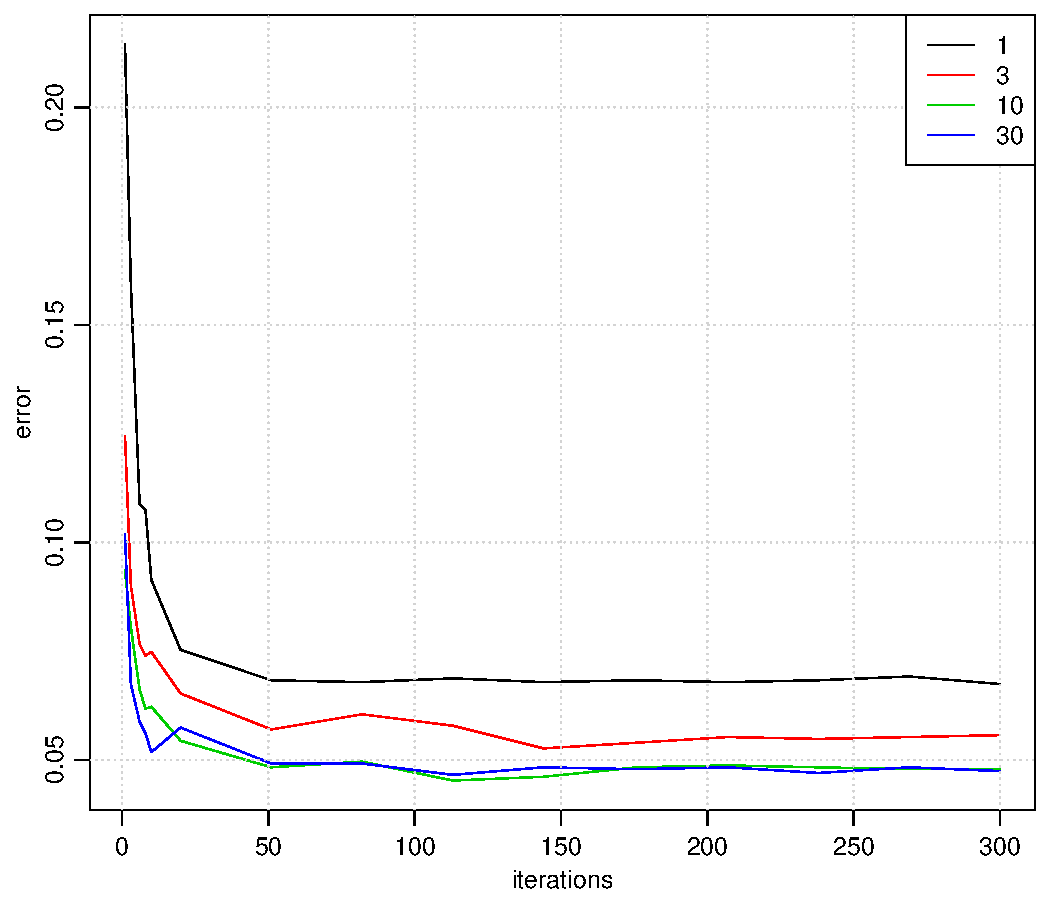
\includegraphics[scale=0.5]{./figures/adaboostSpam.pdf}
\end{center}
\caption{AdaBoost on spam data. For different tree depths.}
\label{fig:adaboostSpam}
\end{figure}

Simulation 2: \\
With and without bootstraping. Maybe include this in Simulation 1.

\subsection{Gradient boosting}
\label{sub:SimGradBoost}
\colorbox{yellow}{Both gradient and stochastic.}\\
\colorbox{yellow}{Problems with gbm. See tutorial}
\url{https://vimeo.com/71992876} \\
\url{http://www.datarobot.com/blog/r-getting-started-with-data-science/}
\\ \colorbox{yellow}{Should I include offset in the model?}
\\ \colorbox{yellow}{Make adaboost with gbm as good as with adabag}
\\ \colorbox{yellow}{Use gbm.fit, as it should be faster for ''power users''} \\
\url{http://www.saedsayad.com/docs/gbm2.pdf} \colorbox{yellow}{Guide to gbm package}\\
\\
Simulation 1:\\
Plot error as function of iterations. This should be done for different shrinkage parameters.\\
Consider plotting training error as well.\\
\\
\begin{figure}[h!]
\begin{center}
    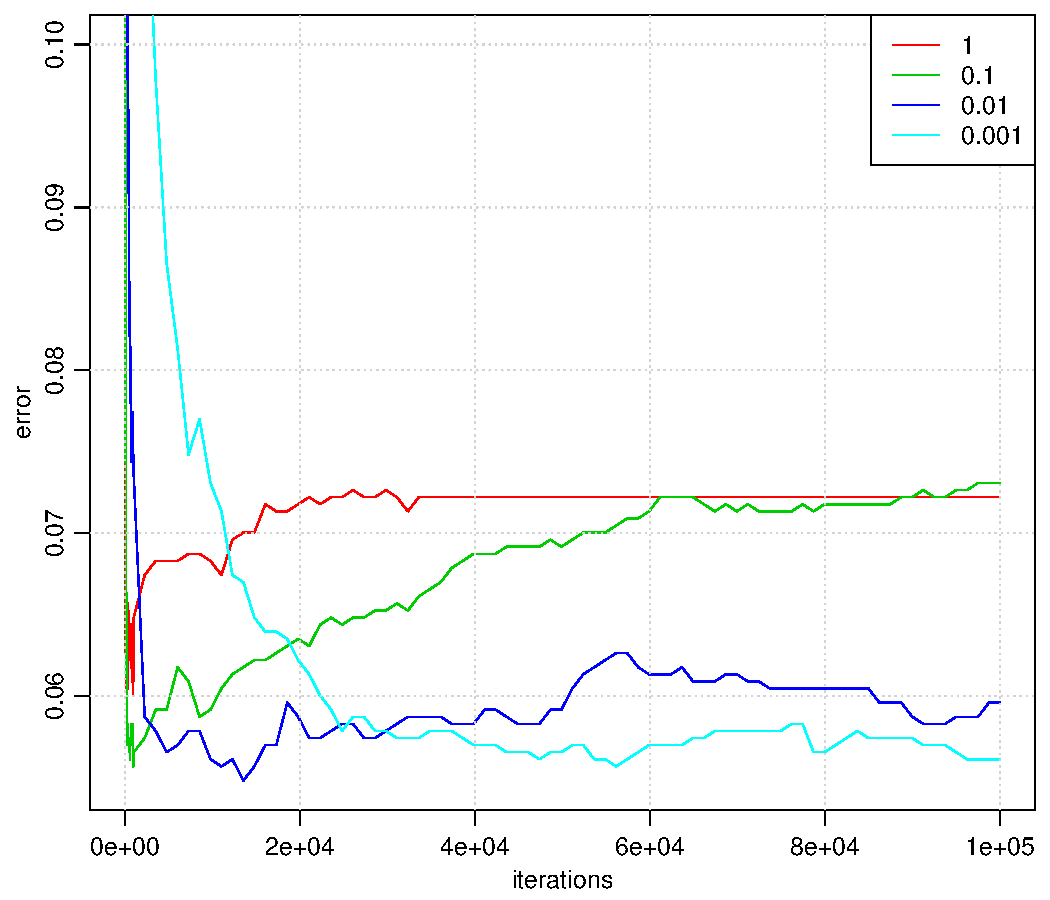
\includegraphics[scale=0.5]{./figures/gradboostSpamShrink2.pdf}
\end{center}
\caption{Gradient boosting on spam data. The shrinkage of each line is specified in the legend.}
\label{fig:gradboostSpamShrink2}
\end{figure}

Simulation 2:\\
Plot error as function of iterations, for different \verb+bag.fractions+, and report time for the different baggigs.\\
\\
\begin{figure}[h!]
  \centering
  \begin{subfigure}[b]{0.48\textwidth}
    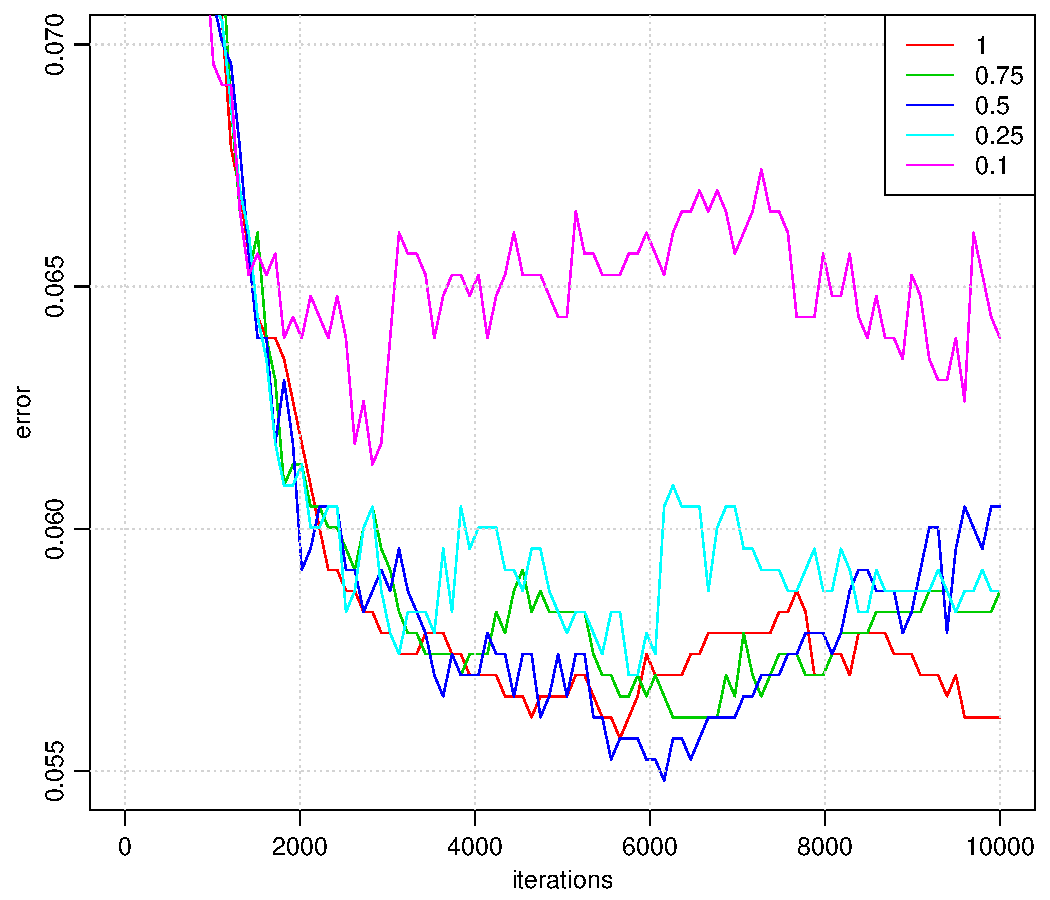
\includegraphics[width=\textwidth]{./figures/gradboostSpamStoch.pdf}
    \caption{Different bootstrap fractions.}
    \label{fig:gradboostSpamStoch}
  \end{subfigure}%
  \quad
  \begin{subfigure}[b]{0.48\textwidth}
    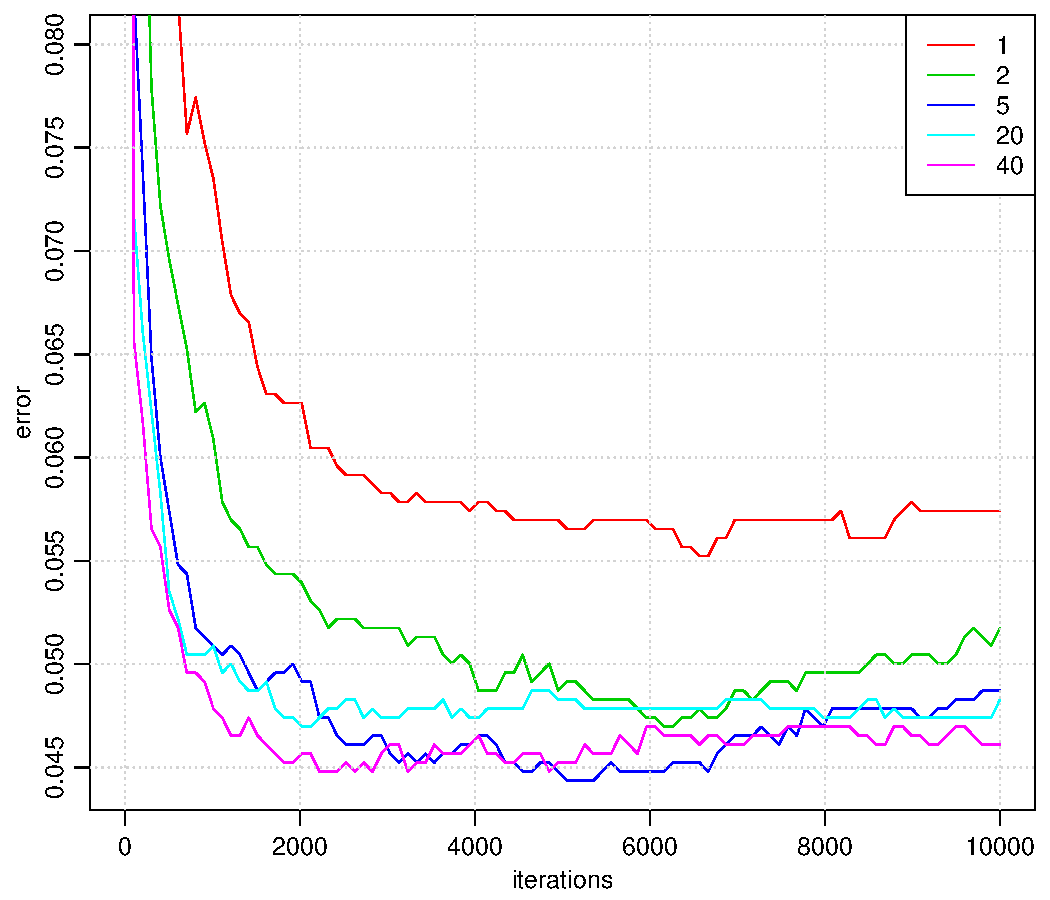
\includegraphics[width=\textwidth]{./figures/gradboostSpamDepth.pdf}
    \caption{Different tree depths.}
    \label{fig:gradboostSpamDepth}
  \end{subfigure}
          %(or a blank line to force the subfigure onto a new line)
  \vspace{1\baselineskip}
  \caption{Stochastic gradient boosting on spam data. Give some parameter values here!!!}
  \label{fig:StochasticGradBoost}
\end{figure}
\todo{parameters in Figure~\ref{fig:StochasticGradBoost}}
\colorbox{yellow}{Comment that there are unusually deep trees in Figure~\ref{fig:gradboostSpamDepth}}

Simulation 3:\\
Use \verb+interaction.depth+ (nr of splits) to set depth of tree, and see how that affect error as function of nr of iteratoins/trees.\\
\\ \colorbox{yellow}{Comment that not additive model as many nodes is better than stumps. See modstat.}
\\ \colorbox{yellow}{Figure~\ref{fig:gradboostSpamDepth}: see p.~13} \url{http://www.stat.cmu.edu/~ryantibs/datamining/lectures/25-boost.pdf}\\


\section{Bagging and Random Forest}
\label{sec:BaggandRFSim}
Simulation 1: \\
Do simulations for bagging with different bootstrap sizes. And the same for random forests\\
\\
\begin{figure}[h!]
  \centering
  \begin{subfigure}[b]{0.48\textwidth}
    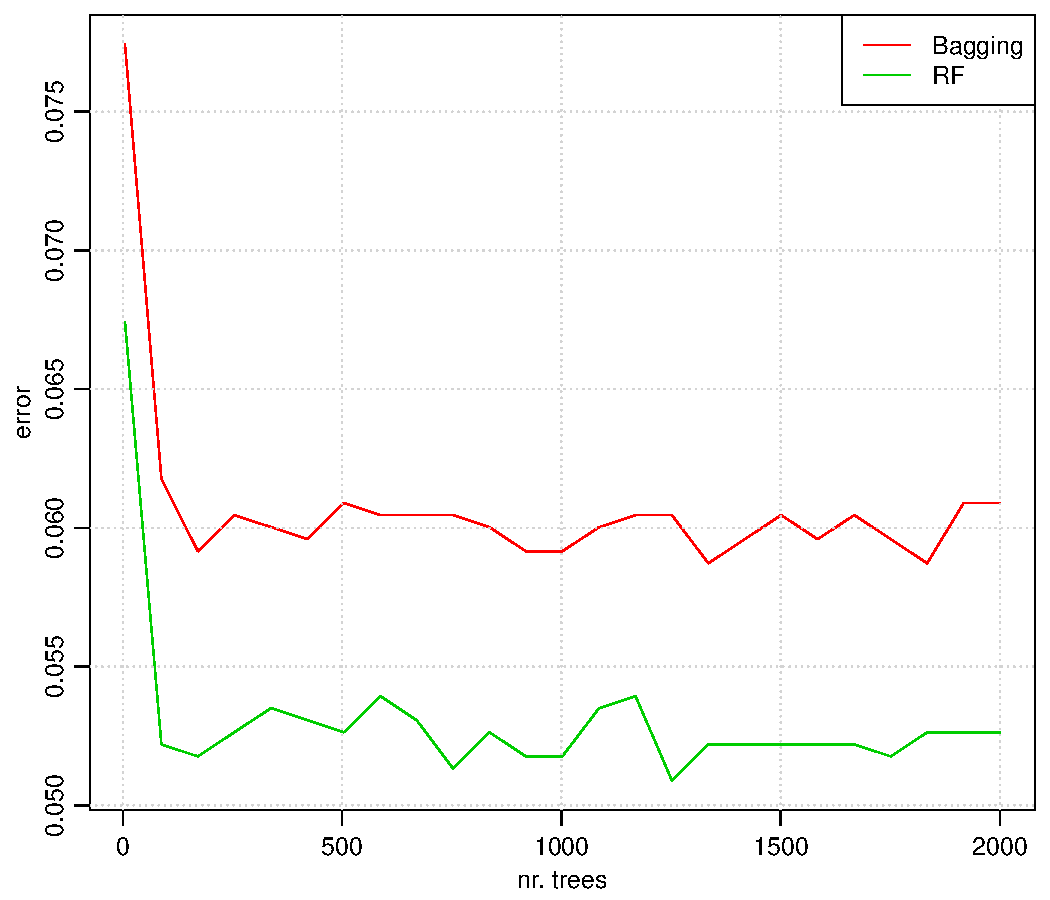
\includegraphics[width=\textwidth]{./figures/baggingAndRFSpam.pdf}
    \caption{Test error as function of bootstrap samples for bagging and RF.}
    \label{fig:baggingAndRFSpam}
  \end{subfigure}%
  \quad
  \begin{subfigure}[b]{0.48\textwidth}
    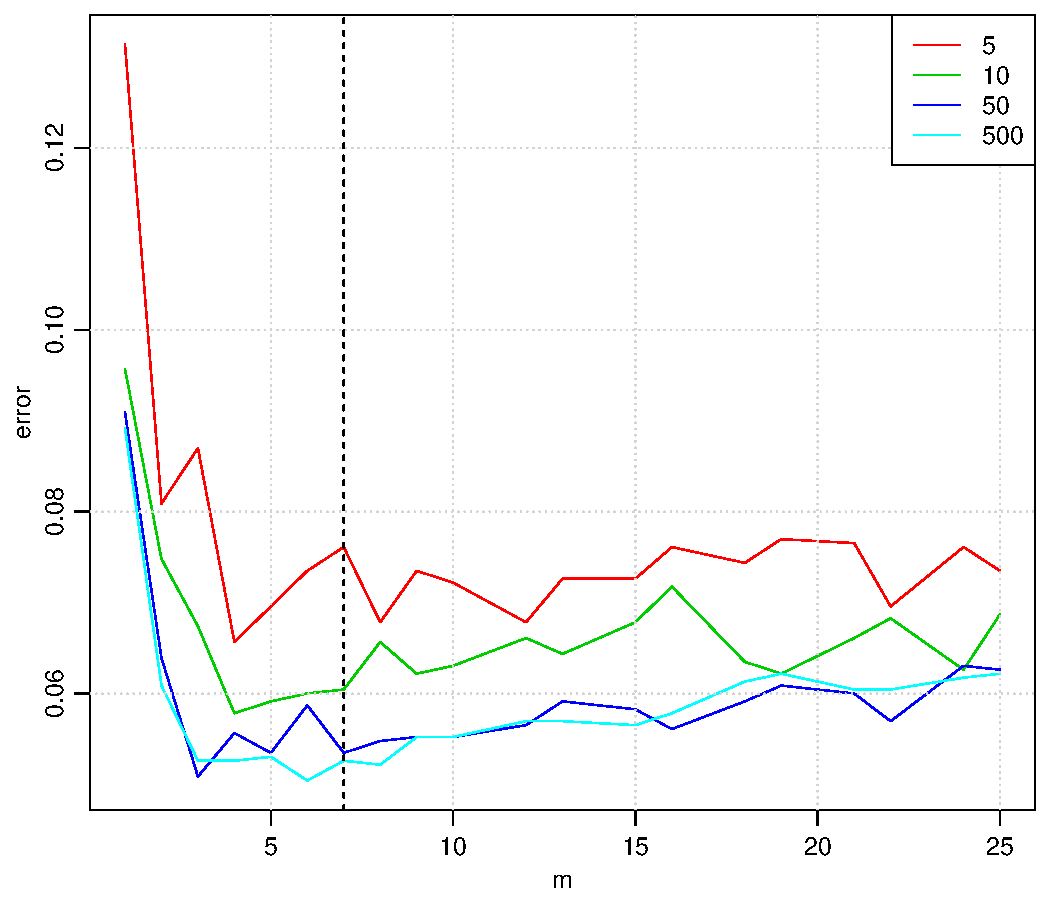
\includegraphics[width=\textwidth]{./figures/RFSpam.pdf}
    \caption{Test error for RF as function of m, for different number of bootstrap samples.}
    \label{fig:RFSpam}
  \end{subfigure}
          %(or a blank line to force the subfigure onto a new line)
  \vspace{1\baselineskip}
  \caption{Misclassification rate for bagging and random forests on spam data.}
  \label{fig:baggAndRF}
\end{figure}
\todo{Comment on line in Figure~\ref{fig:RFSpam}}

Simulation 2: \\
\\
Maybe together with bagging, do simulations for as function of $m$'s, for different bootstrap sizes? \\
\colorbox{yellow}{Not sure what is best here.}\\
\\
\colorbox{yellow}{Comment that Figure~\ref{fig:baggingAndRFSpam} shows how RF don't overfit. Is the same true for bagging?}\\
\\
Simulation 3: \\
Show an example of when bagging and RF fails? If the base classifier is bad, then the aggregated can be bad as well.\\
\colorbox{yellow}{Should I do this?}\\
\\
\colorbox{yellow}{Do simulation to show diffenece between \eqref{eq:aggClass} and \eqref{eq:aggClassP}.}








\section{Compare methods}
\label{sec:Compare methods}
\colorbox{yellow}{Show CART here as well.}

\subsection{Robustness}
\label{sub:Robustness}

\colorbox{yellow}{Add noise to previous test and see how stable the results are.}
\section{Phoneme}
\label{sec:Phoneme}
\colorbox{yellow}{Should I do both at the same time? So do the plots side by side? Or in different sections like now?}

\begin{figure}[h!]
\begin{center}
    \includegraphics[scale=0.5]{./figures/adaboostPhoneme.pdf}
\end{center}
\caption{AdaBoost on Phoneme data. For different tree depths.}
\label{fig:adaboostPhoneme}
\end{figure}

\begin{figure}[h!]
\begin{center}
    \includegraphics[scale=0.5]{./figures/gradboostPhonemeShrink2.pdf}
\end{center}
\caption{Gradient boosting on Phoneme data. The shrinkage of each line is specified in the legend.}
\label{fig:gradboostPhonemeShrink2}
\end{figure}

\begin{figure}[h!]
  \centering
  \begin{subfigure}[b]{0.48\textwidth}
    \includegraphics[width=\textwidth]{./figures/gradboostPhonemeStoch.pdf}
    \caption{Different bootstrap fractions.}
    \label{fig:gradboostPhonemeStoch}
  \end{subfigure}%
  \quad
  \begin{subfigure}[b]{0.48\textwidth}
    \includegraphics[width=\textwidth]{./figures/gradboostPhonemeDepth.pdf}
    \caption{Different tree depths.}
    \label{fig:gradboostPhonemeDepth}
  \end{subfigure}
          %(or a blank line to force the subfigure onto a new line)
  \vspace{1\baselineskip}
  \caption{Stochastic gradient boosting on Phoneme data. Give some parameter values here!!!}
  \label{fig:StochasticGradBoostPhoneme}
\end{figure}

\begin{figure}[h!]
  \centering
  \begin{subfigure}[b]{0.48\textwidth}
    \includegraphics[width=\textwidth]{./figures/baggingAndRFPhoneme.pdf}
    \caption{Test error as function of bootstrap samples for bagging and RF.}
    \label{fig:baggingAndRFPhoneme}
  \end{subfigure}%
  \quad
  \begin{subfigure}[b]{0.48\textwidth}
    \includegraphics[width=\textwidth]{./figures/RFPhoneme.pdf}
    \caption{Test error for RF as function of m, for different number of bootstrap samples.}
    \label{fig:RFPhoneme}
  \end{subfigure}
          %(or a blank line to force the subfigure onto a new line)
  \vspace{1\baselineskip}
  \caption{Misclassification rate for bagging and random forests on Phoneme data.}
  \label{fig:baggAndRFPhoneme}
\end{figure}

